\documentclass{beamer}
% beamer is 128x96 mm
\usepackage{pgf,tikz}
\usepackage{import}
\usepackage{subfig}
\usepackage{float}
\usepackage{xmpmulti}
\usepackage{hyperref}

\usetikzlibrary{arrows}

\title{The Power of Transformations in Geometry}
\author{Ganesh Ajjanagadde \and Shantanu Jain \and James Thomas}
\date{\today}

\begin{document}
\maketitle

\begin{frame}
\frametitle{Block Diagram}
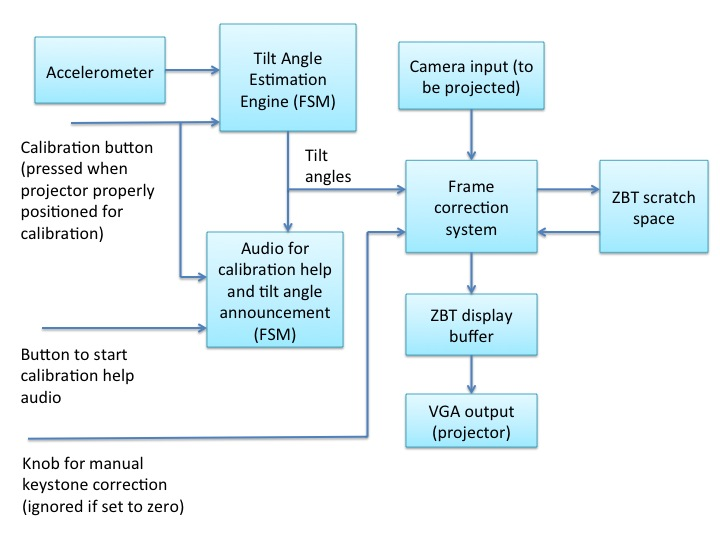
\includegraphics[width=\textwidth]{img/block_diag}
\end{frame}

\begin{frame}
\frametitle{Accelerometer}
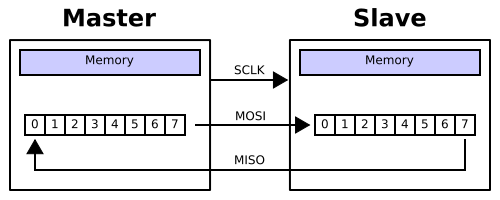
\includegraphics[scale=0.4]{img/spi}
\begin{itemize}
  \item SPI digital interface -- FPGA is master, accelerometer slave
  \item Accelerometer has different registers for x, y, z acceleration, signal which register to read
  \item Configurable SPI clock, but will still need to cross clock domains
  \item Accelerometer nonlinearities -- lookup table needed?
\end{itemize}
\end{frame}

\end{document}
